\documentclass[a4paper,onecolumn,oneside,11pt]{mwrep}
\usepackage[plmath,MeX]{polski}
\usepackage[utf8]{inputenc}
\usepackage{bookman}
\usepackage[T1]{fontenc}
\usepackage{amssymb}  % must be loaded before babel[polish]
\usepackage[polish]{babel}
\usepackage{csquotes}

\DeclareQuoteStyle{polish}
	{\quotedblbase}{\textquotedblright}
	{\quotesinglbase}{\textquoteright}

\usepackage[backend=bibtex,sorting=nyt,style=numeric-comp]{biblatex}
\DeclareLanguageMapping{polish}{src/polish}
\addbibresource{../src/bib.bib} % bibtex is run from inside of build/ directory


\let\emptyset\varnothing

\usepackage{hyperref}
\usepackage{url}
\usepackage{breakurl}

\usepackage{wrapfig}
\usepackage{graphicx}
\usepackage{epstopdf}
\usepackage[subrefformat=parens,labelformat=parens]{subfig}

\usepackage{units}

\usepackage{color}
\definecolor{gray}{rgb}{0.5,0.5,0.5}

\makeatletter

\usepackage{listings}
\usepackage{listingsutf8}
\lstset{
  language=C,
  basicstyle=\small,
  numbers=left,
  numberstyle=\tiny\color{gray},
  stepnumber=1,
  numbersep=5pt,
  showspaces=false,
  showstringspaces=false,
  showtabs=false,
  tabsize=8,
  captionpos=b,
  breaklines=true,
  breakautoindent,
  columns=fixed,
  escapeinside={(*}{*)},
  morekeywords={inline,bool}
}
\renewcommand*\lstlistingname{Wydruk}
\renewcommand*\lstlistlistingname{Spis wydruków}
\def\code{\lstinline[basicstyle=\itshape]}

\usepackage[chapter]{algorithm}
\renewcommand*{\ALG@name}{Algorytm}
\renewcommand*{\listalgorithmname}{Spis algorytmów}
\renewcommand*{\thealgorithm}{\arabic{chapter}.\arabic{algorithm}.}

\usepackage[noend]{algpseudocode}
\renewcommand*{\algorithmicrequire}{\textbf{Wymaga:}}
\renewcommand*{\algorithmicensure}{\textbf{Zapewnia:}}
\renewcommand*{\algorithmiccomment}[1]{{\footnotesize \it \{ #1 \}}}
\renewcommand*{\algorithmicif}{\textbf{Jeżeli}}
\renewcommand*{\algorithmicthen}{}
\renewcommand*{\algorithmicelse}{\textbf{wpp.}}
\renewcommand*{\algorithmicfor}{\textbf{Dla}}
\renewcommand*{\algorithmicforall}{\textbf{Dla wszystkich}}
\renewcommand*{\algorithmicdo}{\textbf{}}
\renewcommand*{\algorithmicwhile}{\textbf{Dopóki}}
\renewcommand*{\algorithmicloop}{\textbf{Wykonuj}}
\renewcommand*{\algorithmicrepeat}{\textbf{Wykonuj}}
\renewcommand*{\algorithmicreturn}{\textbf{zwróć}}
\renewcommand*{\algorithmicuntil}{\textbf{aż}}
\renewcommand*{\algorithmicfunction}{\textbf{Funkcja}}
\renewcommand*{\algorithmicprocedure}{\textbf{Procedura}}

\renewcommand*\lstlistoflistings{%
    \section*{\lstlistlistingname}
    {\secondarysize
    \gdef\previous@toc@level{-1000}%
    \@starttoc{lol}}%
    \if@restonecol\twocolumn\fi
}
\renewcommand*\l@lstlisting{\mw@tocline{1}{0pt}{2.5em}}
\renewcommand*\listoffigures{%
    \section*{\listfigurename}
    {\secondarysize
     \renewcommand*\addvspace[1]{}
    \gdef\previous@toc@level{-1000}%
    \@starttoc{lof}}%
    \if@restonecol\twocolumn\fi
}
\renewcommand*\listofalgorithms{%
    \section*{\listalgorithmname}
    {\secondarysize
    \gdef\previous@toc@level{-1000}%
    \@starttoc{loa}}%
    \if@restonecol\twocolumn\fi
}
\newcommand*\l@algorithm{\mw@tocline{1}{0pt}{2.5em}}

\makeatother

\usepackage[top=2.5cm,bottom=2.5cm,inner=2cm,outer=3cm]{geometry}

\clubpenalty=10000
\widowpenalty=10000
\brokenpenalty=10000
\sloppy

\tolerance4500
\pretolerance250
\hfuzz=1.5pt
\hbadness1450

\renewcommand*{\chaptermark}[1]{\markboth{\scshape\small\bfseries \
#1}{\small\bfseries \ #1}}
\renewcommand*{\sectionmark}[1]{\markboth{\scshape\small\bfseries\thesection.\
#1}{\small\bfseries\thesection.\ #1}}
\newcommand*{\headrulewidth}{0.5pt}
\newcommand*{\footrulewidth}{0.pt}
\pagestyle{uheadings}

\newcommand*{\TODO}[1]{{\setlength{\fboxsep}{0pt}\footnotesize (\colorbox{red}{TODO}: #1)}}
\newcommand*{\ang}[1]{ang.\ {\it #1}}

\usepackage{titling}
\title{Alokacja ciągłych fizycznie obszarów pamięci w~systemie Linux}
\author{Michał Nazarewicz}
\date{\today}
\newcommand*{\theengishtitle}{Physically contiguous memory allocation in Linux-based systems}

\begin{document}

\pagenumbering{roman}
\renewcommand*{\baselinestretch}{1.0}
\raggedbottom

\begin{titlepage}
    % Strona tytułowa
    \vbox to\textheight{\hyphenpenalty=10000
    \begin{center}
        \begin{tabular}{p{107mm} p{9cm}}
            \begin{minipage}{9cm}
              \begin{center}
              Politechnika Warszawska \\
              Wydział Elektroniki i~Technik Informacyjnych \\
              Instytut Informatyki
              \end{center}
            \end{minipage}
            &
            \begin{minipage}{8cm}
            \begin{flushleft}
             \footnotesize
              Rok akademicki 2012/2013
            \vspace*{2.75\baselineskip}
            \end{flushleft}
            \end{minipage} \\
        \end{tabular}
        \vspace*{3.75\baselineskip}
        \par\vspace{\smallskipamount}
        \includegraphics[width=4cm]{build/pw.eps}\par
        \vspace*{2\baselineskip}{\LARGE Praca dyplomowa inżynierska\par}
        \vspace{3\baselineskip}{\LARGE\strut \theauthor\par}
        \vspace*{2\baselineskip}{\huge\bfseries \thetitle\par}

        \vspace*{7\baselineskip}
        \hfill\mbox{}\par\vspace*{\baselineskip}\noindent
        \begin{tabular}[b]{@{}p{3cm}@{\ }l@{}}
            {\large\hfill } & {\large }
        \end{tabular}
        \hfill
        \begin{tabular}[b]{@{}l@{}}
        Opiekun pracy: \\[\smallskipamount]
        {\large dr inż.\ Wojciech Zabołotny}
        \end{tabular}\par
        \vspace*{4\baselineskip}
    \begin{tabular}{p{\textwidth}}
    \begin{flushleft}
        \begin{minipage}{7cm}
        Ocena \dotfill
        \par\vspace{1.6\baselineskip}
        \dotfill
        \par\noindent
        \centerline{\footnotesize Podpis Przewodniczącego} \par
        \centerline{\footnotesize Komisji Egzaminu Dyplomowego}\par
        \end{minipage}
    \end{flushleft}
    \end{tabular}
    \end{center}}

    % Życiorys
    \newpage\thispagestyle{empty}
    \begin{tabular}{p{5cm} p{12cm}}
    \begin{minipage}{5cm}
    \center
    \IfFileExists{bsc-photo.eps}{
      \includegraphics[width=4.5cm]{bsc-photo.eps}
    }{
      \includegraphics[width=4.5cm]{build/photo.eps}
    }
    \end{minipage}
    &
    \begin{minipage}{12cm}
    \begin{flushleft}
    \par\noindent\vspace{1\baselineskip}
    \begin{tabular}[h]{l l}
    {\it Kierunek:}       & Informatyka \\[12pt]
    {\it Specjalność:}    & Inżynieria Systemów \\
                          & Informatycznych \\[12pt]
    {\it Data urodzenia:} & 31 sierpnia 1986~r. \\[12pt]
    {\it Data rozpoczęcia studiów:} & 1 lutego 2006 r. \\
    \end{tabular}
    \par\noindent\vspace{1\baselineskip}
    \end{flushleft}
    \end{minipage}
    \end{tabular}
    \vspace*{1\baselineskip}
    \begin{center}
        {\large\bfseries Życiorys}\par\bigskip
    \end{center}

    \IfFileExists{bsc-bio.tex}{\indent\input{bsc-bio}}{
      \begin{center}
        $\ddot\smile$
      \end{center}
    }
    \par
    \vspace{2\baselineskip}
    \hfill\parbox{15em}{{\small\dotfill}\\[-.3ex]
    \centerline{\footnotesize podpis studenta}}\par
    \vspace{3\baselineskip}
    \begin{center}
        {\large\bfseries Egzamin dyplomowy} \par\bigskip\bigskip
    \end{center}
    \par\noindent\vspace{\baselineskip}
    Złożył egzamin dyplomowy w dn. \dotfill
    \par\noindent\vspace{\baselineskip}
    Z wynikiem \dotfill
    \par\noindent\vspace{\baselineskip}
    Ogólny wynik studiów \dotfill
    \par\noindent\vspace{\baselineskip}
    Dodatkowe wnioski i uwagi Komisji \dotfill
    \par\noindent\vspace{\baselineskip}
    \dotfill

    % Streszczenie
    \newpage\thispagestyle{empty}
    \vspace*{2\baselineskip}
    \begin{center}
        {\large\bfseries Streszczenie}\par\bigskip
    \end{center}

    {\itshape Wiele podzespołów komputera, a~szczególnie
      tzw.\ systemów wbudowanych, jest zazwyczaj podłączonych
      bezpośrednio do magistrali systemowej, przez co muszą operować
      adresami fizycznymi.  Równocześnie mechanizmy bezpośredniego
      dostępu do pamięci (\ang{Direct Memory Access}, \acc{DMA}) są
      ograniczone do transferów sekwencyjnych.  Stwarza to potrzebę,
      alokowania dużych ciągłych fizycznie obszarów pamięci do
      wykorzystania w~takich układach.

      Dotychczas stosowane w~systemach bazujących na jądrze Linux
      rozwiązania wiążą się z~rezerwowaniem dużego obszaru pamięci,
      który wyjęty spod kontroli Linuksa przestaje być użyteczny dla
      jądra i~w~rezultacie jest wykorzystywany nieefektywnie.

      Praca opisuje stworzony przeze mnie alokator pamięci ciągłej,
      \ang{Contiguous Memory Allocator} (\acc{CMA}), który rozwiązuje ten
      problem poprzez zastosowanie mechanizmu migracji, który pozwala
      przenosić zajęte strony i~w~ten sposób tworzyć długie sekwencje
      wolnych stron.}

    \vspace*{1\baselineskip}

    \noindent{\bf Słowa kluczowe}: {\itshape alokacja pamięci, Linux,
      systemy wbudowane.}
    \par
    \vspace{4\baselineskip}
    \begin{center}
        {\large\bfseries Abstract}\par\bigskip
    \end{center}
    \noindent{\bf Title}: {\itshape \theengishtitle}\par
    \vspace*{1\baselineskip}

    {\itshape Many computer components, especially in a~so called
      embedded system, are attached directly to the system bus and thus
      need to operate on physical addresses.  At the same time, Direct
      Memory Access (\acc{DMA}) is limited to sequential transfers only.
      This creates a need to allocate big physically contiguous memory
      buffers to be used with such components.

      Solutions previously used in Linux-based systems boil down to
      reserving a~big memory area which exempted from Linux control
      cannot be used efficiently by the kernel.

      This work describes Contiguous Memory Allocator
      (\acc{CMA})\,---\,an allocator written by me which solves the
      problem by using migration, which makes it possible to move
      allocated pages and thus create a~long sequence of free pages.}
    \vspace*{1\baselineskip}

    \noindent{\bf Key words}: {\itshape memory allocation, Linux,
      embedded systems.}

\end{titlepage}


\tableofcontents

\newpage
\pagenumbering{arabic}
\setcounter{page}{1}

\chapter{Wstęp}

Tematem niniejszej pracy inżynierskiej jest sterownik dla jądra Linux,
który pozwala w~efektywny sposób alokować duże obszary ciągłej
fizycznie pamięci.  Opisanym mechanizmem jest stworzony przeze mnie
alokator ciągłej pamięci, (\ang{Contiguous Memory Allocator}, CMA).

Podstawowym zastosowaniem dużych buforów, który w~głównej mierze
brałem podczas pisania alokatora CMA, jest wykorzystanie ich
w~podzespołach dostępnych w~nowoczesnych telefonach komórkowych.
Niemniej odkąd stworzony przeze mnie kod został dołączony do Linuksa,
różne osoby wykazały zainteresowanie, aby wykorzystywać go również
w~innych celach.


\section{Opis problemu}

W~celu zwiększenia efektywności działania oraz liczby udostępnianych
funkcji, komputery a w~szczególności telefony komórkowe posiadają
wiele wyspecjalizowanych podzespołów.  W~wielu przypadkach, procesor
komunikuje się z~nimi poprzez bufory w pamięci operacyjnej,
przekazując do urządzenia jedynie adresy gdzie dane się znajdują.
Dostęp do RAM-u poprzez takie podzespoły może się jednak wiązać
z~wieloma ograniczeniami.

\begin{figure}[tbp]
  \centering
  \subfloat[System z~układem MMU pomiędzy procesorem a~pamięcią oraz
    urządzeniami podłączonymi bezpośrednie do szyny pamięci.]{
    \label{fig:sys-with-mmu}
    \includegraphics[width=.25\textwidth]{build/mmu-iommu-images--img-nommu.eps}
  } \qquad
  \subfloat[Systemu z~kontrolerem DMA, który pośredniczy w~transferach
    danych pomiędzy pamięcią i~urządzeniami.]{
    \label{fig:sys-with-dma}
    \includegraphics[width=.25\textwidth]{build/mmu-iommu-images--img-dma.eps}
  }\qquad
  \subfloat[Systemu z~zarówno układem MMU jak i~IOMMU, które tłumaczą
    adresy widziane przez odpowiednio procesor oraz urządzenia.]{
    \label{fig:sys-with-iommu}
    \includegraphics[width=.25\textwidth]{build/mmu-iommu-images--img-iommu.eps}
  }
  \caption[Różne przestrzenie adresowe dostępne
    w~komputerze.]{Reprezentacja systemów z~różnymi podzespołami
    uczestniczącymi w~translacji adresów lub transferach danych do
    pamięci operacyjnej.}
  \label{fig:mmu-iommu}
\end{figure}

\subsection{Jednostka translacji adresów}

Nowoczesne architektury przeznaczone do serwerów i~komputerów
osobistych posiadają jednostkę zarządzania pamięcią (\ang{memory
  management unit}, MMU), która tłumaczy adresy logiczne na
fizyczne.  Dzięki temu, bufory, które z~punktu widzenia procesora są
ciągłe, mogą w~rzeczywistości być podzielone na wiele stron
rozrzuconych po pamięci fizycznej.  W~ten sposób, nawet jeżeli program
alokuje wielomegabajtowy obszar, system może zrealizować żądanie
alokując wiele czterokibibajtowych\footnote{Aby uniknąć
  wieloznaczności, stosuję przedrostki „kilo-” i~„mega-” w~znaczeniu
  odpowiednio tysiąc i~milion (zgodnie z~układem SI), a~„kibi-”
  i~„mebi-” w~znaczeniu odpowiednie $2^{10} = 1024$ i~$2^{20}$
  (zgodnie z~tzw.\ przedrostkami ICE).} stron i~nie przejmować się
fragmentacją pamięci.

\subsection{Bezpośredni dostęp do pamięci}

Niemniej, tak jak to przedstawia rysunek \subref*{fig:sys-with-mmu},
jednostka MMU przeważnie nie jest dostępna dla pozostałych układów
znajdujących się w~urządzeniu, takich jak np.\ karta dźwiękowa, czy
kontroler sieciowy.  Na szczęście także i~dla tych przypadków istnieje
rozwiązanie w~postaci mechanizmu bezpośredniego dostępu do pamięci
(\ang{Direct Memory Access}, DMA), którego celem jest odciążenie
procesora od przesyłania danych.  Co prawda urządzenie nadal znajduje
się w~przestrzeni adresów fizycznych, co ilustruje rysunek
\subref*{fig:sys-with-dma}, ale dzięki układowi DMA nieciągłość
buforów może zostać przed nim ukryta.

Układ DMA może obsługiwać technikę wektorowego wejścia/wyjścia
(\ang{vectored I/O}), która pozwala zbierać wiele rozrzuconych
fragmentów danych w~jeden bufor (stąd też inna nazwa:
rozrzucanie/zbieranie, \ang{scatter/gather}).  Nawet jeżeli DMA nie
umożliwia wykorzystania tej techniki, procesor może ją symulować
poprzez sekwencyjne wywoływanie wielu mniejszych transferów, choć jest
to niestety mniej efektywne rozwiązanie.

Mechanizm bezpośredniego dostępu do pomięci jest jednak ograniczony do
transferów sekwencyjnych.  Sprawdza się bardzo dobrze dla operacji
dyskowych, ale nie nadaje się dla sprzętowego dekodera wideo, który
potrzebuje dostępu do wielu dekodowanych ramek
jednocześnie.\footnote{Jednym z~rodzajów ramek stosowanych do
  kodowania klatki ze strumienia wideo jest b-ramka, która już nawet
  w~starszych standardach takich jak MPEG-2 może odwoływać się do
  jednej poprzedzającej i~jednej następującej klatki, a w~przypadku
  nowszego standardu H.264, może zależeć od więcej niż dwóch innych
  ramek.}

\subsection{IOMMU}

Oczywiście nie ma żadnych technologicznych przeszkód do zastosowania
jednostki translacji adresów również dla podzespołów innych niż
procesor.  Istotnie istnieją platformy sprzętowe z~tzw.\ MMU
wejścia/wyjścia (IOMMU), który pozwala na budowanie dużych ciągłych
buforów złożonych ze stosunkowo małych stron.  W~takich systemach
w~zasadzie nie ma (lub nie powinno być) konieczności alokowania
wielomegabajtowych buforów.

Niestety, nawet jeżeli układ IOMMU jest dostępny, jego obecność może
się wiązać z~dodatkowym kosztem wynikającym z~nieoptymalnego kodu
(\textcite{bib:price-of-safety} pokazuje zwiększenie zużycia procesora
wynikające z~nieoptymalnego mapowania o~15-30\%) lub konieczności
odczytywania mapowań z~pamięci
(\textcite{bib:mitigate-iotlb-bottleneck} pokazuje, że przy
nieoptymalnych odczytach, czas dostępu do pamięci w~buforach rzędu
\unit[1]{MiB} może wynieść nawet 45\%).  Z~tego względu architekt
platformy może zdecydować się wyłączyć IOMMU i~rozwiązać problem
„w~oprogramowaniu”.

\subsection{Podsumowanie}

Z~uwagi na koszty i~ograniczenia zarówno kontrolerów DMA jak i~układów
MMU, w~wielu systemach wbudowanych, takich jak np.\ telefony
komórkowe, takie mechanizmy są często niedostępne.  Jednocześnie,
właśnie takie urządzenia posiadają dużo wyspecjalizowanych
podzespołów, jak chociażby aparat fotograficzny, czy układ do
szybkiego dekodowania obrazów JPEG.

Powoduje to, że tego typu układy muszą operować bezpośrednio na
adresach fizycznych i~w~konsekwencji, wszelkie stosowane przez nie
bufory muszą być ciągłe w~pamięci fizycznej.  Niestety, Linux nie jest
dobrze przystosowany do alokowania takich
obszarów.\footnote{W~szczególności, Linux nie jest nawet w~stanie (bez
  modyfikowania źródła) zarządzać obszarami większymi niż cztery
  mebibajty (1024 strony), gdy tymczasem pięciomegapikselowa kamera
  potrzebuje buforu o~rozmiarze 15 megabajtów, a~pojedyncza ramka
  \ang*{full HD} (tj.\ 1920 $\times$ 1080) zajmuje ponad sześć
  megabajtów.}


\section{Możliwe rozwiązania}

Ponieważ opisany powyżej problem jest znany od dawna, na przestrzeni
lat powstało wiele rozwiązań programowych umożliwiających obejście
trudność w~alokacji dużych obszarów.  W~tym podrozdziale opiszę je
pokrótce oraz przedstawie ich ograniczenia.

\subsection{Przypisywanie pamięci na stałe}

Najprostszym, i~stosunkowo często stosowanym, rozwiązaniem jest
rezerwacja przy starcie systemu pewnego regionu pamięci na potrzeby
konkretnych sterowników.

Najłatwiejszym, acz niezbyt eleganckim sposobem jest wykorzystanie
argumentu \code|mem| jądra.  Przekazany przez program rozruchowy
powoduje, że Linux nie stara się automatycznie wykryć dostępnej
w~systemie pamięci RAM i~zamiast tego interpretuje przekazane
informacje.  W~ten sposób, możliwe jest ograniczenie widzianej przez
system pamięci, tak że ukryte regiony mogą być wykorzystywane przez
konkretne sterowniki.

Bardziej eleganckim rozwiązaniem jest skorzystanie z~alokatora
memblock, który jest aktywny zanim jądro zainicjuje wszystkie swoje
podsystemy.  Jego zadaniem jest śledzenie wolnej pamięci zanim jeszcze
bardziej zaawansowany alokator stron będzie dostępny w~systemie.
Wołany dostatecznie wcześnie, jest w~stanie zaalokować duże obszary
pamięci, które potem można wykorzystać w~dowolny sposób.

Niestety, o~ile tego typu rozwiązania mogą być wystarczające, jeżeli
podzespoły wymagają stosunkowo małych buforów lub jeżeli pamięć jest
cały czas wykorzystywana (np.\ w~przypadku bufora ramki,
\ang{framebuffor}), przestaje się on skalować przy współczesnych
systemach, gdyż wymaga rezerwacji wielu megabajtów pamięci, która
przez większość czasu nie jest do niczego wykorzystywana.

\subsection{Pula pamięci fizycznej}\label{sec:intro-pmm}

Bardziej skomplikowanym rozwiązaniem jest mechanizm, który rezerwuje
pewną przestrzeń pamięci, ale zamiast na stałe przypisywać obszary do
urządzeń, pozwala sterownikom alokować bufory, wtedy, gdy są one
potrzebne.

W~trakcie moich prac stworzyłem \ang*{Physical Memory Manager} (PMM)
\autocite{patch:pmm}, który implementuje dokładnie te założenia. W~tym
podstawowym zastosowaniu, PMM nie przedstawia sobą nic nowego.  Już
bowiem w~1996 roku Matt Welsh napisał pierwszą wersję dodatku
\ang*{bigphysarea} dla jądra 1.3.71, który był z~różnym zaangażowaniem
utrzymywany i~przystosowywany aż do wersji 3.2 Linuksa
\autocite{patch:bigphys}.

PMM posiadał jednak wiele dodatkowych funkcji opisanych w~podrozdziale
\ref{sec:evo-pmm}, których próżno szukać w~\ang*{bigphysarea}, czy
w~innych dostępnych poprawkach do jądra.  Niemniej, pomimo swoich
dodatkowych funkcji, nie rozwiązywał do końca problemu nieefektywnego
wykorzystania pamięci, przez co nie został przyjęty przez społeczność
programistów Linuksa i~musiałem rozwijać inne rozwiązanie.

\subsection{Zarys Contiguous Memory Allocatora}

Ostatecznym rozwiązaniem stał się alokator ciągłej pamięci (CMA),
który umożliwia systemowi używanie zarezerwowanej pamięci, o~ile żadne
urządzenie jej w~danym momencie nie potrzebuje.

W~swoich początkowych wersjach, również mechanizm CMA działał na
założeniach podobnych do PMM\,---\,rezerwował przy starcie systemu
pamięć, którą potem zarządzał pozwalając sterownikom i~programom na
alokowanie obszarów ciągłych fizycznie \autocite{patch:cma-1}.

Wynika to z~faktu, iż pierwsze wersje alokatora CMA skupiały się
w~dużej mierze na rozwiązywaniu problemu przypisywania różnych
zarezerwowanych obszarów do różnych urządzeń, a~także umożliwianiu
sterownikom alokowanie różnych buforów w~różnych obszarach pamięci, co
opisałem w~podrozdziale \ref{sec:evo-cma}.

Z~czasem, coraz bardziej integrowałem mechanizm CMA z~kodem
zarządzania pamięci w~Linuksie w~wyniku czego, pamięć rezerwowana przy
starcie systemu, stała się dostępna dla reszty systemu, o~ile żaden
sterownik jej nie używał \autocite{patch:cma-24}.  Takie rozwiązanie
zostało ostatecznie zaakceptowane przez społeczność deweloperów
Linuksa i~jest dostępne w~źródłach Linuksa począwszy od wersji 3.5.
W~tej pracy opisuję alokator CMA w~formie w~jakiej znalazł się on
w~Linuksie 3.5\footnote{Należy zauważyć, że Linux jest szybko
  rozwijającym się projektem wolnego oprogramowania i~ponieważ
  mechanizm CMA używana jest przez coraz więcej osób, jest ona ciągle
  rozwijana i~im dalej w~przyszłość, tym bardziej opis w~niniejszej
  pracy będzie się różnił od stanu faktycznego.}.

\section{Wielkie strony}

Zagadnieniem związanym w~pewnym stopniu z~mechanizmem CMA są wielkie
strony (\ang{huge pages}).  O~ile zwyczajne strony pamięci mają
przeważnie cztery kibibajty, o~tyle wielkie strony mają rozmiary rzędu
dwóch lub czterech mebibajtów\footnote{Konkretne rozmiary zależą od
  architektury procesora i~co więcej wiele rozmiarów może być
  dostępnych jednocześnie.}.  Stosowane są w~celu zmniejszenia liczby
wpisów w~tablicy translacji adresów, a~co za tym idzie również TLB
procesora.

Począwszy od wersji 2.6.38, Linux posiada mechanizm automatycznego
wykorzystywania wielkich stron dla działających programów,
\ang{transparent huge pages} \autocite{bib:v2.6.38}.  Dzięki niemu,
o~ile to możliwe, wiele czterokibibajtowych stron mapowanych jest za
pomocą pojedynczego wpisu w~tablicy translacji adresów.

Podobnie jak w~przypadku alokatora CMA, wymaga to alokowania dużych
obszarów ciągłych fizycznie.  Tym co różni oba mechanizmy jest wymóg
aby alokacja CMA zakończyła się sukcesem i~do tego w~jak najkrótszym
czasie, gdy tymczasem automatyczne wykorzystywanie wielkich stron jest
procesem oportunistyczny i~jeżeli w~danej chwili w~systemie nie ma
dostatecznie dużego wolnego obszaru, mechanizm ten nie zostanie
wykorzystywany.

Z~uwagi na te odmienne wymagania, obie implementacje, pomimo, że
pozornie mające podobne założenia, są w~dużym stopniu rozłączne.

\chapter{Sposób użycia CMA}\label{sec:cma-usage}

Pomimo, że idea CMA jest stosunkowo prosta, mechanizm ten urósł do
raczej skomplikowanego interfejsu, który integruje się dość głęboko
z~systemem zarządzania pamięci jądra Linuksa.  Pomimo tego, jego
użycie nie jest szczególnie trudne, a~w~wielu przypadkach autor
sterownika, który chciałby korzystać z~CMA nie musi niczego zmieniać
w~swoim kodzie.

\section{Wykorzystanie w~sterownikach}\label{sec:usage-drivers}

CMA integruje się z~interfejsem programowania DMA (DMA API), co
oznacza, że jeżeli CMA jest włączone i~zintegrowane z~daną
architekturą, poprawnie napisany sterownik (tzn.\ taki, który korzysta
z~DMA API) będzie korzystał z~CMA bez konieczności dokonywania
jakichkolwiek zmian.

Tak naprawdę, sterowniki nie powinny odwoływać się bezpośrednio do
funkcji CMA, gdyż są one zbyt nisko poziomowe i~operują na stronach,
gdy tymczasem sterowniki urządzeń są raczej zainteresowane adresami
szyny.\footnote{W~ogólności, adres szyny strony może być inny niż jej
  adres fizyczny i~DMA API zostało zaprojektowane tak, aby brać to pod
  uwagę.}  Co więcej, CMA nie posiada żadnych mechanizmów
gwarantujących spójność pamięci podręcznej -- zadanie to leży
w~kwestii DMA API.

Najprostszym mechanizmem z~tego interfejsu są funkcje
\code|dma_alloc_coherent| i~\code|dma_free_coherent|.  Służą one
odpowiednio do alokacji i~zwalniania buforów DMA, których zawartość
jest zawsze spójna z~tym co widzi procesor\footnote{W~różnych
  architekturach efekt ten jest uzyskiwany w~różny sposób.
  W~architekturze Intel istnieje gwarancja spójność zawartości kości
  RAM oraz pamięci podręcznej procesora, gdy tymczasem architektura
  ARM nie daje takich gwarancji.  Z~tego powodu, w~systemach opartych
  o~Linuksa działających na platformie ARM, bufory alokowane przy
  pomocy \code|dma_alloc_coherent| nie podlegają buforowaniu w~pamięci
  podręcznej procesora.}.  Wydruk \ref{lst:dma-alloc-example} pokazuje
sposób wykorzystania tych dwóch funkcji.  Prosty sterownik, który
można wykorzystać do testowania CMA można znaleźć
w~\cite{patch:cma-test}, a~dokładniejszy opis DMA API w~rozdziale 15
\cite{bib:ldd3}.

\begin{lstlisting}[float=tbhp,caption={Alokacja bufora DMA z~użyciem
      DMA API.},label=lst:dma-alloc-example]
static struct device *my_dev;

void *my_dev_alloc_buffer(unsigned long size_in_bytes, dma_addr_t *dma_addrp)
{
	void *virt_addr;

	virt_addr = dma_alloc_coherent(my_dev, size_in_bytes,
				       dma_addrp, GFP_KERNEL);
	if (!virt_addr)
		dev_err(my_dev, "Unable to allocate %lu-byte DMA %buffer",
			size_in_bytes);
	return virt_addr;
}

void *my_dev_free_buffer(unsigned long size_in_bytes,
			 void *virt_addr, dma_addr_t dma_addr)
{
	dma_free_coherent(my_dev, size_in_bytes, virt_addr, dma_addr);
}
\end{lstlisting}


\section{Integracja z~architekturą procesora}\label{sec:integrate-with-arch}

CMA działa dzięki rezerwowaniu w~trakcie startu systemu pewnego
regionu pamięci (zwanego regionem CMA), który po zainicjowaniu całego
mechanizmu CMA jest zwracany do systemu (tak że może być
wykorzystywany do pewnego rodzaju alokacji).  Aby taki obszar został
zarezerwowany, w~trakcie startu systemu musi zostać wywołana funkcja:

\begin{lstlisting}
void dma_contiguous_reserve(phys_addr_t limit);
\end{lstlisting}

Wywołanie to musi nastąpić gdy podsystem alokacji pamięci czasu startu
systemu (tj.\ {\it. memblock}) zostanie zainicjowany, ale przed
aktywowaniem alokatora stron.  Dla przykładu w~architekturze ARM
dogodnym miejscem jest funkcja \code|arm_memblock_init|, a~x86
-- \code|setup_arch| zaraz po aktywowaniu memblock.

Argument \code|limit| określa górny adres pamięci fizycznej,
którego zarezerwowany obszar CMA nie przekroczy.  Dzięki niemu regiony
CMA mogą zostać ograniczone do adresów dostępnych dla urządzeń
w~systemie.  Przykładowo w~architekturze ARM argument ten przyjmuje
wartość zmiennych \code|arm_dma_limit| lub
\code|arm_lowmem_limit|, którakolwiek jest mniejsza,
a~w~procesorach 64-bitowych może zaistnieć potrzeba ograniczenia do
32-bitowych adresów.  Jeżeli wartością tego argumentu jest zero, na
region CMA nie jest narzucany żaden limit.

Ilość zarezerwowanej pamięci zależy od argumentu \code|cma|
(który określa rozmiar regionu w~bajtach) przekazywanego do jądra
w~trakcie startu, lub, jeżeli argumentu tego nie ma, ustawień
kompilacji jądra.  W~trakcie konfiguracji kompilacji jądra można
wybrać jeden z~czterech sposobów określania rozmiaru:

\begin{enumerate}
\item stały rozmiar wyrażony w~bajtach,
\item rozmiar wyrażony w~procentach całkowitej pamięci dostępnej
  w~systemie,
\item większe z~pierwszych dwóch opcji, lub
\item mniejsze z~pierwszych dwóch opcji.
\end{enumerate}

Domyślną wartością konfiguracji jest alokacja \unit[16]{MiB}.

Funkcja \code|dma_contiguous_reserve| tworzy domyślny region
CMA wykorzystywany przez wszystkie urządzenia, które nie mają
przypisanych prywatnych regionów CMA.  Prywatne regiony CMA opisane są
w~podrozdziale \ref{sec:priv-regions}.


\subsection{Poprawki specyficzne dla architektury}

Na niektórych architekturach może zaistnieć przeprowadzenia dodatkowej
obróbki zarezerwowanych regionów pamięci.

Przykładowo, z~uwagi na brak spójności pamięci RAM i~pamięci
podręcznej procesora na architekturze ARM, wymagane jest aby strony,
z~których korzystają urządzenia, były mapowane jako niepodlegające
buforowaniu (\ang{noncacheable}).  Co więcej, specyfikacja
architektury mówi, że jeżeli dana strona jest mapowana z~różnymi
parametrami buforowania (\ang{cacheability}), efekt działania systemu
nie jest zdefiniowany.

Dlatego w~architekturze ARM, kod integrujący CMA z~DMA API zmienia
mapowanie strony na niechachewalne na czas, gdy jest ona używana przez
urządzenie.

Z~drugiej strony, aby przyśpieszyć translację adresów, jądro stara się
stosować tak zwane wielkie strony.  Pozwala to zmapować \unit[2]{MiB}
pamięci (512 normalnych stron o~rozmiarze \unit[4]{KiB}) poprzez jeden
wpis w~tablicy mapowania.

Niestety, takie mapowanie uniemożliwia zmianę parametrów mapowania
pojedynczej strony.  Z~uwagi na to, regiony CMA są przygotowane w~ten
sposób, że mapowanie wielkich stron jest rozbijane na wiele mapowań
pojedynczych stron co pozwala na (w~miarę) proste modyfikowanie
ustawień cachowania danej strony.  Więcej na ten temat można
przeczytać w~artykule \cite{bib:cma-and-arm}.

Aby to umożliwić, dla każdego regionu CMA, zawołana zostanie funkcja

\begin{lstlisting}
void dma_contiguous_early_fixup(phys_addr_t base, unsigned long size);
\end{lstlisting}

Nie jest ona zdefiniowana przez CMA i~musi zostać dostarczona przez
kod danej architektury.  Jej deklaracja powinna znaleźć się w~pliku
nagłówkowym \code|asm/dma-contiguous.h|.  Jeżeli funkcjonalność
ta nie jest konieczna, wystarczy dostarczyć pustą implementację
(np.\ prezentowaną przez wydruk \ref{lst:empty-fixup}).

\begin{lstlisting}[float=tbhp,caption={Plik nagłówkowy
      \code|asm/dma-contiguous.h| z~pustą implementacją funkcji
      \code|dma_contiguous_early_fixup|.},label=lst:empty-fixup]
#ifndef ASM_DMA_CONTIGUOUS_H
#define ASM_DMA_CONTIGUOUS_H

#ifdef __KERNEL__

#include <linux/types.h>
#include <asm-generic/dma-contiguous.h>

static inline void
dma_contiguous_early_fixup(phys_addr_t base, unsigned long size)
{
	/* nop, no need for early fixups */
}

#endif
#endif
\end{lstlisting}

Należy pamiętać, że funkcja ta jest wołana dość wcześnie w~trakcie
startu systemu, zatem wiele podsystemów może jeszcze nie być
dostępnych, a~w~szczególności funkcja \code|kmalloc| nie będzie
działać.  Co więcej, może ona zostać wywołana kilkakrotnie, dla
różnych regionów CMA, ale nie więcej niż \code|MAX_CMA_AREAS|
razy (domyślnie 8).

\subsection{Integracja z~podsystemem DMA}\label{sec:usage-integrate}

Aby sterowniki mogły korzystać z~CMA poprzez DMA API, CMA musi zostać
dodane do podsystemu DMA danej architektury.  Alokacja bufora CMA
odbywa się poprzez wywołanie funkcji:

\begin{lstlisting}
struct page *dma_alloc_from_contiguous(
	struct device *dev,
	int count,
	unsigned int align);
\end{lstlisting}

Pierwszym argumentem jest urządzenie na rzecz którego odbywa się
alokacja.  Drugim jest \emph{liczba stron} do zaalokowania.

Trzeci argument to wyrównanie alokacji wyrażone w~rzędzie strony, lub
innymi słowy, jeżeli bufor ma być wyrównany do $a$ bajtów, parametr
\code|align| powinien przyjąć wartość $\log_2 a - \log_2
\mathrm{PAGE\_SIZE}$ (lub dla stron o~rozmiarze \unit[4096]{KiB}:
$\log_2 a - 12$).  Jeżeli żadne wyrównanie nie jest wymagane, należy
zwyczajnie przekazać zero -- zmniejszy to również problem
z~fragmentacją.  Warto zauważyć, że na wartość argumentu
\code|align| nałożone jest ograniczenie
\code|CONFIG_CMA_ALIGNMENT|, który jest ustawiane w~trakcie
kompilacji jądra.  Jego domyślną wartością jest osiem (co oznacza
wyrównanie do 256 stron).

Funkcja \code|dma_alloc_from_contiguous| zwraca wskaźnik na
pierwszą stronę spośród serii \code|count| zaalokowanych stron,
lub \code|NULL| w~przypadku nieudanej alokacji.

Do zwolnienia bufora wykorzystywana jest funkcja:

\begin{lstlisting}
bool dma_release_from_contiguous(
	struct device *dev,
	struct page *pages,
	int count);
\end{lstlisting}

Argumenty \code|dev| i \code|count| mają takie samo
znaczenie jak w~funkcji \code|dma_alloc_from_contiguous|,
a~argument \code|pages| jest wartością zwróconą przez tę funkcję.

Jeżeli dany bufor nie był zaalokowany poprzez CMA, funkcja
\code|dma_release_from_contiguous| zwróci \code|false|.
W~przeciwnym wypadku, bufor zostanie zwolniony i~funkcja zwróci
\code|true|.  Ta zwracana wartość może zostać wykorzystana przez
DMA API aby rozróżnić, czy dany bufor jest buforem CMA, czy też nie.

Wydruk \ref{lst:dma-integration} pokazuje fragment patcha, który
integruje CMA z~podsystemem DMA architektury x86.

\begin{lstlisting}[float=tbhp,caption={Integracja CMA z~podsystemem DMA
      architektury x86.},label=lst:dma-integration]
diff --git a/arch/x86/kernel/pci-dma.c b/arch/x86/kernel/pci-dma.c
@@ -99,14 +99,18 @@ void *dma_generic_alloc_coherent(
 				 dma_addr_t *dma_addr, gfp_t flag)
 {
	(*{\it [ \ldots ]}*)
 again:
-	page = alloc_pages_node(dev_to_node(dev), flag, get_order(size));
+	if (!(flag & GFP_ATOMIC))
+		page = dma_alloc_from_contiguous(dev, count, get_order(size));
+	if (!page)
+		page = alloc_pages_node(dev_to_node(dev), flag, get_order(size));
 	if (!page)
 		return NULL;
@@ -126,6 +130,16 @@ again:
 	return page_address(page);
 }

+void dma_generic_free_coherent(struct device *dev, size_t size, void *vaddr,
+			       dma_addr_t dma_addr)
+{
+	unsigned int count = PAGE_ALIGN(size) >> PAGE_SHIFT;
+	struct page *page = virt_to_page(vaddr);
+
+	if (!dma_release_from_contiguous(dev, page, count))
+		free_pages((unsigned long)vaddr, get_order(size));
+}
+
\end{lstlisting}

\paragraph{Alokacje w~kontekście atomowym} \hspace{0pt} \\

Należy pamiętać, iż funkcja \code|dma_alloc_from_contiguous|
nie może zostać wywołana w~kontekście atomowym (np.\ z~procedury
obsługi przerwania), a~jednocześnie dopuszczalne jest wywołanie
\code|dma_alloc_coherent| z~kontekstu atomowego.  Z~tego
powodu, subsystem DMA musi posiadać inny mechanizm przeznaczony dla
takich alokacji.

Najprostszym rozwiązaniem jest zarezerwowanie pewnego, stosunkowo
niewielkiego, obszaru pamięci, przeznaczonego do alokacji w~kontekście
atomowym.  Istniejące architektury muszą posiadać tego typu
mechanizmy.


\section{Regiony CMA dla poszczególnych urządzeń}\label{sec:priv-regions}

Po dokonaniu zmian opisanych w~powyższym podrozdziale, sterowniki
urządzeń powinny już działać.  Korzystając z~DMA API odwołują się
bowiem do CMA.

Jednak niektóre urządzenia mogą mieć specyficzne wymagania.  Dla
przykładu, wielo-formatowy koder multimedialny (\ang{Multi-format
  codec}, MFC) znajdujący się na platformie S5PV110 wymaga, aby bufory
na różne dane, znajdowały się w~różnych bankach pamięci (co pozwala na
dostęp do danych przez dwa kanały zwiększając tym sposobem
przepustowość pamięci).  Ponadto, zależnie od istniejących na
platformie urządzeń, wskazane może być izolowanie pewnych grup
urządzeń.  Dla przykładu mieszanie alokacji dla stosunkowo małych
tekstur dla koprocesora graficznego z~alokacjami dużych buforów
przeznaczonych dla kamery, może przyczynić się do zwiększenia
fragmentacji regionu CMA.

Funkcja \code|dma_declare_contiguous| tworzy domyślny region
CMA, ale istnieje możliwość przypisania różnych regionów CMA do
poszczególnych urządzeń.  Istnieje mapowanie wiele-do-jednego pomiędzy
strukturą \code|device|, a~regionem CMA.  Oznacza to, że
pojedynczy region CMA może zostać przypisany do danego urządzenia, ale
jeżeli urządzenie ma korzystać z~wielu regionów CMA konieczne jest
stworzenie kilku struktur \code|device|.

\paragraph{Przypisywanie regionu CMA do pojedynczego urządzenia} \hspace{0pt} \\

Aby przypisać region CMA do urządzenia wystarczy wywołać funkcję:

\begin{lstlisting}
int dma_declare_contiguous(
	struct device *dev,
	unsigned long size,
	phys_addr_t base,
	phys_addr_t limit);
\end{lstlisting}

Pierwszy argument to urządzenie do którego region ma być przypisany.
Drugi to \emph{rozmiar w~bajtach}.  Trzeci to adres gdzie region ma
się zaczynać lub zero, jeżeli nie ma to znaczenia.  Ostatni argument,
\code|limit|, ma takie samo znaczenie jak w~przypadku funkcji
\code|dma_contiguous_reserve|.  Dla przykładu, wydruk
\ref{lst:s5p-priv-region} pokazuje fragment patcha dodającego prywatne
regiony do dwóch urządzeń.

Istnieje limit „prywatnych” regionów CMA, konkretnie
\code|CONFIG_CMA_AREAS|, którego domyślna wartość to siedem.
Jeżeli limit ten zostanie przekroczony, funkcja
\code|dma_declare_contiguous| zacznie zwracać
\code|-ENOSPC|.  Jednakże, jeżeli istnieje taka potrzeba, nic nie
stoi na przeszkodzie aby ten limit zwiększyć w~trakcie kompilacji
jądra.

% For some reason, breaklines=true does not work, so I'm breaking the
% line manually...
\begin{lstlisting}[float=tbhp,caption={Przypisanie prywatnych regionów
      CMA do dwóch urządzeń.},label=lst:s5p-priv-region]
diff --git a/arch/arm/plat-s5p/dev-mfc.c b/arch/arm/plat-s5p/dev-mfc.c

 void __init s5p_mfc_reserve_mem(phys_addr_t rbase, unsigned int rsize,
 				phys_addr_t lbase, unsigned int lsize)
 {
	(*{\it [ \ldots ]}*)
+	if (dma_declare_contiguous(&amp;s5p_device_mfc_r.dev, (*{\color{gray} $\hookleftarrow$}*)
(*{\color{gray} $\hookrightarrow$}*)		rsize, rbase, 0))
+		printk(KERN_ERR "Failed to reserve memory for MFC device (*{\color{gray} $\hookleftarrow$}*)
(*{\color{gray} $\hookrightarrow$}*)			(\%u bytes at 0x\%08lx)\n",
+		       rsize, (unsigned long) rbase); (*{\color{gray} $\hookleftarrow$}*)
(*{\color{gray} $\hookrightarrow$}*)	(*{\it [ \ldots ]}*)
+	if (dma_declare_contiguous(&amp;s5p_device_mfc_l.dev, (*{\color{gray} $\hookleftarrow$}*)
(*{\color{gray} $\hookrightarrow$}*)		lsize, lbase, 0))
+		printk(KERN_ERR "Failed to reserve memory for MFC device (*{\color{gray} $\hookleftarrow$}*)
(*{\color{gray} $\hookrightarrow$}*)			(\%u bytes at 0x\%08lx)\n",
+		       rsize, (unsigned long) rbase);
 }
\end{lstlisting}

\paragraph{Przypisywanie jednego regionu CMA do wielu urządzeń} \hspace{0pt} \\

Odrobinę bardziej skomplikowane jest przypisanie tego samego regionu
do kilku urządzeń.  Obecny interfejs CMA nie udostępnia funkcji, która
by na to pozwalała, ale i~tak nie jest to szczególnie trudne do
osiągnięcia.  Wystarczy zastosować metodę opisaną powyżej, aby
przypisać region do jednego urządzenia, a~następnie skopiować ten
region do drugiego urządzenia.  Całą sekwencja powinna zostać wykonana
jako \code|postcore_initcall|.  Poniższy kod pokazuje jak taki
efekt może zostać osiągnięty:

\begin{lstlisting}
static int __init foo_set_up_cma_areas(void) {
	struct cma *cma = dev_get_cma_area(device1);
	dev_set_cma_area(device2, cma);
	return 0;
}
postcore_initcall(foo_set_up_cma_areas);
\end{lstlisting}

\paragraph{Brak domyślnego regionu} \hspace{0pt} \\

Warto zauważyć, że nic nie stoi na przeszkodzie, aby nie tworzyć
domyślnego regionu CMA.  Oczywiście, jeżeli nie zostanie on stworzony,
urządzenia, którym nie zostaną przypisane prywatne regiony nie będą
mogły korzystać z~buforów CMA.

\chapter{Zapoznanie z~alokatorem stron}

Ponieważ mechanizm CMA w~dużym stopniu integruje się z~podsystemem
zarządzania pamięci (\ang{memory management} lub w~skrócie mm), do
jego zrozumienia potrzeba ogólnej wiedzy na temat tego w~jaki sposób
jądro śledzi i~przydziela pamięć procesom i~sterownikom.

Linux posiada wiele mechanizmów alokacji pamięci.  Począwszy od
najprostszych w~użyciu funkcji \code|kmalloc| i \code|vmalloc|,
poprzez mechanizmy puli pamięci, aż do alokatora czasu bootowania
i~alokatorów pamięci dostępnej dla urządzeń zewnętrznych
\autocite[rozdział 8]{bib:ldd3}.  Pomimo tak dużej liczby interfejsów,
wiele z~nich sprowadza się do wywołania alokatora stron (\ang{page
  allocator}), który jest sercem podsystemu zarządzania pamięcią.
Uproszczone zależności między tymi komponentami przedstawia rysunek
\ref{fig:allocators-base}.

\section{Algorytm bliźniaków}

Alokator stron implementuje algorytm bliźniaków (skąd też jego inna
angielska nazwa: {\it buddy system} lub {\it buddy allocator}), który
operuje na blakach o~rozmiarze $2^k$ jednostek.  W~przypadku Linuksa
jednostką jest pojedyncza strona fizyczna, a~na $k$~narzucone jest
ograniczenie $k < \mathrm{MAX\_ORDER}$.  \code|MAX_ORDER| może
zależeć od architektury, na którą Linux jest kompilowany, ale
zazwyczaj ma wartość $11$ (toteż na potrzeby tej pracy zakładam, iż $0
\le k \le 10$).

\begin{wrapfigure}{o}[1.5cm]{0.3\textwidth}
\begin{center}
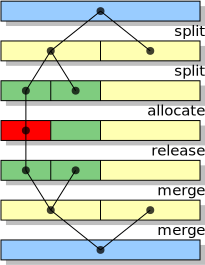
\includegraphics[width=0.25\textwidth]{build/alloc-free-cycle.eps}
\end{center}
\caption[Zarządzanie pamięcią w~algorytmie bliźniaków]{Graficzna
  reprezentacja cyklu alokacji i~zwalniania buforów w~algorytmie
  bliźniaków.}
\end{wrapfigure}

W~Linuksie, przez $k$ rozumie się rząd strony (\ang{page order}).
Strona rzędu 0 to pojedyncza strona fizyczna, strona rzędu 1
(\ang{1-order page}) to dwie strony fizyczne itd.\ aż do strony rzędu
10, czy też strony maksymalnego rzędu (\ang{max order page}), która
składa się z~1024 stron fizycznych.  Ogólnie, strona rzędu $n$ składa
się z~dwóch stron rzędu $n-1$.

Funkcja \code|alloc_pages|, która jest interfejsem dla alokatora
stron, przyjmuje jako argument właśnie rząd żądanej strony.  Wynikają
stąd następujące właściwości alokatora stron:

\begin{itemize}
\item Nie można za jego pomocą zaalokować mniej niż jednej strony,
  tj.\ 4096 bajtów.
\item Interfejs nie pozwala alokować obszarów, których rozmiar nie
  jest potęgą dwójki.
\item Gdyby jednak chcieć zaalokować taki obszar, wiązałoby się to
  z~potencjalnie dużą fragmentacją wewnętrzną.  Dla przykładu kolorowa
  tekstura o~rozmiarze $512 \times 512$ pikseli zajmuje
  \unit[768]{KiB}, zatem bufor ją przechowujący musiałby mieć rozmiar
  \unit[1]{MiB}, z~których \unit[256]{KiB}, a~więc \nicefrac{1}{4},
  byłoby nieużywane.
\item Alokator stron nie jest w~stanie zaalokować obszaru większego
  niż \unit[4]{MiB}.  Z~tego powodu, nie nadaje się do alokowania
  ciągłego fizycznie buforu dla pięciomegapikselowej kamery, czy nawet
  pojedynczej ramki {\it full HD}.
\end{itemize}

\begin{figure}[tbp]
  \centering
  \includegraphics[width=\textwidth]{build/linux-allocators--base.eps}
  \caption[Alokatory dostępne w~jądrze Linux.]{Relacje między kilkoma
    najistotniejszymi alokatorami pamięci dostępnymi w~Linuksie.}
  \label{fig:allocators-base}
\end{figure}

Jak zatem działa algorytm bliźniaków?  Alokator posiada listę wolnych
stron, których rząd jest pomiędzy $0$ a~$10$.  W~Linuksie zrealizowane
jest to poprzez 11 list dwukierunkowych, gdzie każda przeznaczona jest
dla stron o~konkretnym rzędzie.

Gdy sterownik chce zaalokować stronę rzędu $n$, alokator sprawdza
odpowiednią listę.  Jeżeli jest ona pusta, przechodzi do listy ze
stronami rzędu $n+1$, aż znajdzie wolną stronę (lub dojdzie do
maksymalnego rzędu, co sygnalizuje nieudaną alokację.  Jeżeli uzyskana
w~ten sposób strona ma rząd większy niż żądany, jest ona dzielona na
pół, aż do osiągnięcia żądanego rozmiaru.  Strony, które powstały na
skutek podziału większej strony na pół, nazywamy stronami
bliźniaczymi.  Cały proces ilustruje algorytm \ref{alg:buddy-alloc}

\begin{algorithm}
\caption[Alokacja strony w~algorytmie bliźniaków.]{Alokacja strony
  rzędu $k$ w~algorytmie bliźniaków.}
\label{alg:buddy-alloc}
\begin{algorithmic}[1]
\Require $0 \leq k < \mathrm{MAX\_ORDER}$
\Function{AllocatePage}{$k$}
    \State $i \gets k$
    \While {lista stron rzędu $i = \emptyset$}
        \State $i \gets i + 1$
        \If {$i = \mathrm{MAX\_ORDER}$}
            \State \Return $\emptyset$
        \EndIf
    \EndWhile

    \State $p \gets$ strona z listy stron rzędu $i$
    \While {$i \neq k$}
        \State $i \gets i - 1$
        \State podziel $p$ na pół na $p_1$ i $p_2$
        \Comment{Strony $p_1$ i $p_2$ nazywamy stronami bliźniaczymi}
        \State $p \gets p_1$
        \State dodaj $p_2$ do listy stron rzędu $i$
    \EndWhile
    \State \Return $p$
\EndFunction
\end{algorithmic}
\end{algorithm}

Przy zwalnianiu, dopóki to możliwe, strona jest łączona ze swoją
bliźniaczą stroną, dzięki czemu strony są dodawane do listy wolnych
stron o~dużym rzędzie.  Proces ten ilustruje algorytm
\ref{alg:buddy-free}

\begin{algorithm}
\caption[Zwalnianie strony w~algorytmie bliźniaków.]{Zwalnianie strony
  $p$ rzędu $k$ w algorytmie bliźniaków.}
\label{alg:buddy-free}
\begin{algorithmic}[1]
\Procedure{FreePage}{$p$, $k$}
    \While {$k + 1 \neq \mathrm{MAX\_ORDER} \wedge p$ posiada wolną stronę bliźniaczą}
        \State $p' \gets$ strona bliźniacza $p$
        \State usuń $p'$ z~listy wolnych stron
        \State $k \gets k + 1$
        \State $p~\gets$ strona powstała w~wyniku połączenia $p$ i~$p'$ \label{alg:buddy-free:join}
    \EndWhile
    \State dodaj $p$ do listy wolnych stron rzędu $k$ \label{alg:buddy-free:add}
\EndProcedure
\end{algorithmic}
\end{algorithm}

Dokładniejszy opis algorytmu bliźniaków oraz przedstawienie jego
właściwości można znaleźć na stronach 435--455
\autocite{bib:taocp-fa}, a~jego zastosowanie w~Linuksie w~podrozdziale
8.1.7 \autocite{bib:utlk}.


\section{Migracja i~typy migracji}\label{sec:migratetype}

Kolejnym istotnym elementem alokatora stron pominiętym z~opisu
w~poprzednim podrozdziale są typy migracji (\ang{migratetype}),
których jest sześć: {\it unmovable}, {\it reclaimable}, {\it movable},
{\it cma}, {\it reserve} oraz {\it isolate}).

\begin{itemize}
\item Dla potrzeb tej pracy traktuję typy {\it unmovable}, {\it
  reclaimable} i~{\it reserve} jak jeden typ -- typ nieruchomy.  To
  uproszczenie wynika z~faktu, iż dla mechanizmu CMA istotne jest
  tylko rozróżnienie pomiędzy stronami ruchomymi i~nieruchomymi.
\item Strony które są typu ruchomego charakteryzują się tym, że ich
  adres fizyczny nie jest istotny, w~związku z~czym mogą być
  przeniesione w~inne miejsce pamięci RAM.
\item Typ {\it cma} jest nowym typem dodanym dla potrzeb interfejsu
  CMA i~jest opisany dokładniej w~podrozdziale \ref{sec:migrate-cma}.
\item Typ {\it isolate} jest niejako pseudo-typem, gdyż jeżeli wolna
  strona ma taki typ, nie może ona zostać zaalokowana.  Więcej na
  temat sposobu w~jaki ten typ może być wykorzystywany opisuję
  w~podrozdziale \ref{sec:alloc-contig-range}.
\end{itemize}

Jednym z~przykładów stron ruchomych są strony anonimowe działających
procesów.  Ponieważ program odwołują się do nich poprzez mapowania
wirtualne, o~ile tablice translacji zostaną uaktualnione, zawartość
strony może być przeniesiona w~dowolne inne miejsce.  Podobnie wygląda
sprawa z~buforami dyskowymi i~wieloma innymi strukturami, którymi
zarządza jądro.

Proces przenoszenia ruchomej strony nazywa się migracją
i wykorzystywany jest między innymi przy obsłudze hot-swapu pamięci,
a~także w~trackie procesu zagęszczania \autocite{bib:compaction,
  bib:supporting-large-contig-regions}, którego celem jest zwiększenie
liczby dostępnych stron o~wysokich rzędach.

\begin{algorithm}
\caption[Migracja strony.]{Migracja strony $p$.}
\label{alg:migrate}
\begin{algorithmic}[1]
\Procedure{MigratePage}{$p$}
    \State $p' \gets$ \Call{AllocPage}{$0$}
    \State skopiuj zawartość $p$ do $p'$
    \State uaktualnij odwołania do $p$ tak aby wskazywały na $p'$
    \State \Call{FreePage}{$p$, $0$}
\EndProcedure
\end{algorithmic}
\end{algorithm}

Najbardziej skomplikowanym krokiem migracji -- zilustrowanej poprzez
algorytm \ref{alg:migrate} -- jest uaktualnienie odwołań do strony
tak, aby wskazywały na nową stronę $p'$.  Ponieważ istnieje wiele
rodzajów stron ruchomych (strony anonimowe, bufory dyskowe itp.), jest
to krok specyficzny dla danej strony.

Przykładowo dla stron anonimowych wiąże się to z~uaktualnieniem
tablicy translacji adresów tak, aby wskazywały w~nowe miejsce, a~także
wyczyszczeniem pamięci TLB (\ang{Translate Lookaside Buffer}), aby nie
posiadała, żadnych nieaktualnych wpisów.

Wołając funkcję \code|alloc_pages|, typ migracji strony jest
przekazywany jako argument, co pozwala alokatorowi stron grupować
strony tego samego typu.  Jest to istotne, gdyż mechanizm zagęszczania
nie działa zbyt dobrze jeżeli ruchome strony przelatają się
z~pozostałymi stronami, które nie podlegają migracji.


\section{Grupy stron}

Grupowanie stron realizowane jest poprzez podział pamięci na bloki
(\ang{pageblock}) składające się z~\code|pageblock_nr_pages| stron
(czy też równoważnie na bloki rzędu \code|pageblock_order|).
Konkretne wartości tych stałych zależą od architektury, no którą jądro
zostało skompilowane, jak i~opcji konfiguracyjnych wybranych w~trakcie
kompilacji.  Niemniej przeważnie wartość tych stałych to odpowiednio
1024 (stron) i~(rząd) 10 i~właśnie takie są przyjęte w~tej pracy
i~wykorzystane w~graficznej reprezentacji na rysunku \ref{fig:pages}.

\begin{figure}[tbp]
\begin{center}
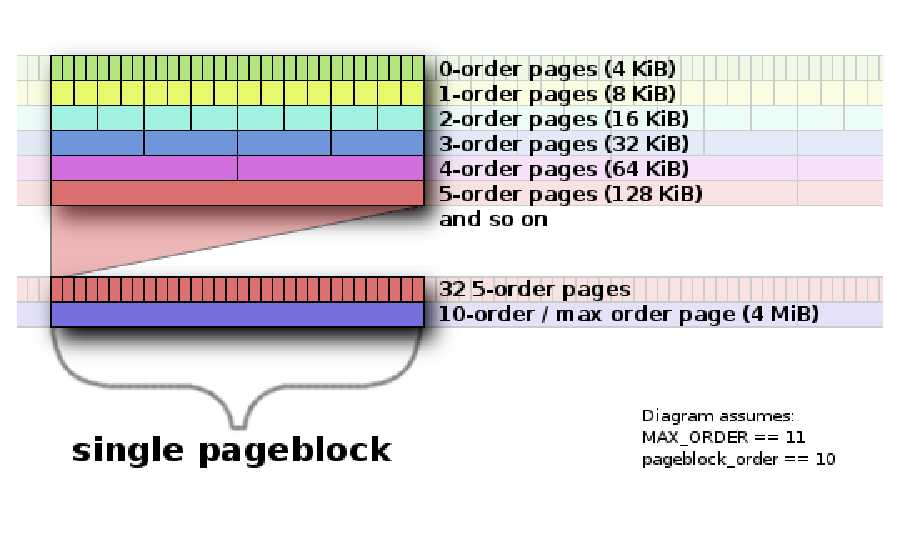
\includegraphics[width=0.8\textwidth]{build/pages.eps}
\end{center}
\caption[Organizacja pamięci w~Linuksie.]{Graficzna reprezentacja
  organizacji stron pamięci stosowanej w~podsystemie zarządzania
  pamięcią Linuksa.}
\label{fig:pages}
\end{figure}

Każdy blok stron (\ang{pageblock}) ma przypisany typ migracji,
a~alokator stron posiada oddzielne listy wolnych stron dla każdego
typu migracji.  Zatem patrząc na algorytm \ref{alg:buddy-alloc} należy
zdawać sobie sprawę, iż rozpatruje on listy wolnych stron danego typu
migracji.

\section{Zmiana typu migracji}\label{sec:type-change}

Należy pamiętać, iż dla jądra zrealizowanie alokacji jest ważniejsze
od trzymania stron o~tym samym typie migracji razem.  Dlatego dla
każdego typu migracji istnieje lista zapasowych (\ang{fallback}) typów
migracji.  Jeżeli alokacja dla żądanego typu migracji nie powiedzie
się, alokator stron będzie próbował z~kolejnymi typami z~list, tak jak
to pokazuje algorytm \ref{alg:buddy-fallback}

Co więcej, jeżeli rząd żądanej strony jest dostatecznie duży, typ
migracji wszystkich wolnych stron w~danym bloku zostaje zmieniano na
ten zgodny z~wywołaniem funkcji \code|alloc_pages|.

\begin{algorithm}
\caption[Alokacja z~uwzględnieniem typu migracji.]{Alokacja strony
  rzędu $k$ z~uwzględnieniem typu migracji $m$}
\label{alg:buddy-fallback}
\begin{algorithmic}[1]
\Function{ChangeBlockMigrateType}{$b$, $m$}
\State zmień typ migracji $b$ na $m$
\ForAll {wolnych stron $p' \in b$}
    \State przenieś $p'$ na listę wolnych stron typu $m$
\EndFor
\EndFunction
\Statex
\Function{AllocPageMigrateType}{$k$, $m$}
    \State $f \gets$ lista zapasowych typów migracji dla typu $m$
    \State dodaj $m$ na początek $f$
    \ForAll{$m' \in f$}
        \State $p \gets$ \Call{AllocPage}{$k$} biorąc pod uwagę listy stron typu $m'$
        \If {$p \neq \emptyset$}
            \If {$m \neq m' \wedge k \geq \nicefrac{\mathrm{page\_order}}{2}$}
                \State $b \gets$ blok stron zawierający $p$
                \State \Call{ChangeBlockMigrateType}{$b$, $m$}
            \EndIf
            \State \Return $p$
        \EndIf
    \EndFor
    \State \Return $\emptyset$
\EndFunction
\end{algorithmic}
\end{algorithm}

Podczas zwalniania, gdy strona jest dodawana do listy wolnych stron
(wideczne w~linii \ref{alg:buddy-free:add} algorytmu
\ref{alg:buddy-free}) typ migracji listy, na którą strona trafia
determinowany jest poprzez typ migracji przypisany blokowi stron do
którego dana strona należy.

Istotne jest tutaj, aby zauważyć, iż bloki stron mogą zmieniać swój
typ migracji, a~także, że nawet jeżeli blok ma dany typ migracji,
strony o~innym typie migracji mogą być z~niego przydzielone.


\section{Listy PCP}\label{sec:pcp-lists}

Ostatnim istotnym, z~punktu widzenia mechanizmu CMA, aspektem
alokatora stron są listy PCP (\ang{per CPU pages})
\autocite[podrozdział 8.1.8]{bib:utlk}.  Ponieważ listy wolnych stron
są współdzielone w~obrębie całego systemu dostęp do nich musi być
synchronizowany pomiędzy wszystkimi procesorami.  Aby uniknąć kosztów
związanych z~synchronizacją, każdy procesor posiada swoje prywatne
listy PCP, na których znajdują się wolne strony rzędu 0.  Biorąc
również i~ten aspekt pod uwagę, alokacja przyjmuje postać
przedstawianą w~algorytmie \ref{alg:buddy-pcp}

\begin{algorithm}
\caption[Alokacja z~uwzględnieniem list PCP.]{Alokacja strony rzędu
  $k$ z~typem migracji $m$ z~uwzględnieniem list PCP.}
\label{alg:buddy-pcp}
\begin{algorithmic}[1]
\Function{AllocPageUsePCP}{$k$, $m$}
    \If {$k \neq 0$}
        \State $p \gets$ \Call{AllocPageMigrateType}{$k$, $m$}
    \Else
        \State $l \gets$ lista PCP dla typu migracji $m$
        \If {$l = \emptyset$}
            \State $i \gets 0$
            \Repeat
                \State $p \gets$ \Call{AllocPageMigrateType}{$0$, $m$}
                \If {$p \neq \emptyset$}
                    \State dodaj $p$ do $l$
                    \State $i \gets i + 1$
                \EndIf
            \Until {$i \geq n \vee p = \emptyset$} \Comment{Wartość
              $n$ jest zależna od różnych czynników}
        \EndIf
        \If {$l = \emptyset$}
            \State \Return $\emptyset$
        \Else
            \State $p \gets$ pierwsza strona z $l$
            \State usuń pierwszą stronę z $l$
            \State lista PCP dla typu migracji $m$ $\gets l$
        \EndIf
    \EndIf
    \State \Return $p$
\EndFunction
\end{algorithmic}
\end{algorithm}


\section{Inne aspekty alokatora stron}

Powyższy opis pomija wiele szczegółów alokatora stron, które nie są
istotne z~punktu widzenia mechanizmu CMA.  Niemniej dla porządku
wymienię kilka istotniejszych detali, które wpływają w~dużej mierze na
sposób w~jaki Linux zarządza pamięcią.

Po pierwsze cała pamięć podzielona jest na strefy (\ang{zones})
\autocite[podrozdział 8.1.3]{bib:utlk}, których, zależnie od
architektury oraz opcji kompilacji, może być pięć:

\begin{description}
\item[ZONE\_DMA] Strefa przeznaczona dla urządzeń, które nie są
  w~stanie wykonywać transferów DMA w~całej przestrzeni adresowej.  Na
  przykład w~architekturze x86 strefa ta jest przeznaczona dla
  urządzeń ISA, które operują na 24-bitowy adresach.
\item[ZONE\_DMA32] Strefa przeznaczona dla urządzeń operujących
  na 32-bitowych adresach pracujących w~architekturze x86\_64.
\item[ZONE\_NORMAL] Strefa z~„normalnymi” stronami, które są na
  stałe zmapowane w~przestrzeni adresowej jądra.
\item[ZONE\_HIGHMEM] Strefa ze stronami, dla których zabrakło
  adresów logicznych w~przestrzeni jądra i~które nie posiadają stałego
  mapowania.
\item[ZONE\_MOVABLE] Strefa, z~które można alokować jedynie
  strony ruchome.
\end{description}

Co więcej, pamięć jest również podzielona na węzły (\ang{nodes}),
które odpowiadają wezłom w~systemach z~niejednolitym dostępem do
pamięci (\ang{Non-Uniform Memory Access} lub NUMA)
\autocite[podrozdział 8.1.2]{bib:utlk}.  Ponieważ w~architekturach
tego typu czas dostępu do pamięci zależy od jej miejsca względem
procesora, istotne jest alokowanie buforów blisko procesora, który
bódzie z~nich korzystał.

Niniejszy rozdział przemilczał również co się dzieje jeżeli podczas
alokacji wolna pamięć nie może zostać odnaleziona.  Otóż jeżeli
algorytm \ref{alg:buddy-alloc} nie znajdzie żadnej wolnej strony
aktywowana jest tzw.\ wolna ścieżka (\ang{slow path}), która
wykorzystuje różne mechanizmy odzyskiwania pamięci (np.\ poprzez
zwalnianie buforów dyskowych, czy w~najgorszym przypadku zabiciu
jednego z~działających procesów, czego dokonuje {\it out-of-memory
  killer} lub OOM {\it killer}) \autocite[rozdział 17]{bib:utlk}.

Istnieje jeszcze wiele innych aspektów takich -- jak chociażby
alokacja w~kontekście atomowym (np.\ w~trakcie obsługi przerwania),
tzw.\ wskaźniki poziamu wody (\ang{watermarks}), które kontrolują jak
duży wolnej pamięci jest w~systemie -- które wprowadzają dodatkową
komplikację do podsystemu zarządzania pamięcią, jednak ponieważ nie
mają one wpływu na mechanizm CMA, wychodzą poza zakres niniejszej
pracy w~związku z~czym są całkowicie ignorowane.

\section{Implementacja i~sposób działania mechanizmu CMA}

Podstawowym założeniem alokatora CMA jest umożliwienie alokowania
dużych obszarów ciągłych fizycznie bez konieczneści rezerwacji na
wyłączność dużej ilości pamięci.  Aby to umożliwić, interfejs CMA
korzysta z~mechanizmu migracji stron opisanego pokrótce w~podrozdziale
\ref{sec:migratetype}.  Ogólny zarys alokacji z~regionów CMA
przedstawiony jest na rysunku \ref{fig:cma-alloc-algo} a~niniejszy
rozdział opisze ją w~większych szczegółach.

\begin{figure}[tbp]
  \includegraphics[width=\textwidth]{build/cma-alloc-algo.eps}
  \caption{Schemat działania alokatora CMA.}
  \label{fig:cma-alloc-algo}
\end{figure}


\subsection{Typ migracji CMA}\label{sec:migrate-cma}

Migracja jest możliwa tylko dla stron ruchomych.  Niestety, przed
zaimplementowaniem alokatora CMA, Linux nie posiadał mechanizmu, który
pozwalałby zagwarantować istnienia dużego obszaru, w~którym strony są
albo wolne, albo ruchome.  Ponieważ (jak opisałem w~podrozdziale
\ref{sec:type-change}) jądro dopuszcza alokacje nieruchomych stron
z~bloków ruchomych, a~także posiada mechanizm na skutek którego bloki
zmieniają swój typ, aby mechanizm CMA mógł działać poprawnie, należało
stworzyć nowy typ migracji -- nazwanym po prostu typem migracji CMA --
który posiada dwie bardzo istotne cechy: (i) z~bloków oznaczonych
typem CMA mogą być alokowane tylko strony ruchome, oraz (ii) blok
oznaczony typem CMA nie zmienia swojego typu (na skutek działania
alokatora stron).

O~ile pierwsza właściwość jest stosunkowo prosta do osiągnięcia,
zagwarantowania niezmienności typu bloku stron wymagało
zidentyfikowania wszystkich sytuacji, w~których blok może zmienić swój
typ (a~także sytuacji, w~których strony mogą trafić na listy wolnych
stron dla typu niezgodnego z~typem bloku, do którego należą) i~dodanie
odpowiednich warunków zapewniających, że niepożądana zmiana nie
nastąpi.

\subsection{Alokowanie wybranego obszaru pamięci}\label{sec:alloc-contig-range}

W~sytuacji, gdy istnieje gwarancja, że dany zakres stron posiada
jedynie strony wolne i~ruchome, można przystąpić do jej alokacji.
Drugim krokiem implementowania alokatora CMA było zatem stworzenie
funkcji, która dostaje jako argument zakres stron, a~następnie migruje
wszystkie zajęte strony, a~wolne usuwa z~listy wolnych stron.  Właśnie
to czyni funkcja \code|alloc_contig_range|.

Pierwszym krokiem wykonywanym przez tę funkcję jest zmiana typu bloków
stron na izolowany typ migracji.  Pomimo, że izolowane strony są
przechowywane na liście wolnych stron i~są pod kontrolą alokatora
stron, nie są one używano do zaspokajania żądań alokacji.  W~ten
sposób, funkcja \code|alloc_contig_range| uzyskuje gwarancje, że
w~trakcie jej działania strony, na których operuje nie zostaną
zaalokowane dla innych wątków jądra.

W~dalszej części wołana jest kolejna stworzona przeze mnie funkcja
\code|__alloc_contig_migrate_range|, której zadaniem jest
zidentyfikowanie i~zmigrowanie wszystkich zajętych stron z~podanego
zakresu.  Funkcja ta szukac stron, które mogą zostać zmigrowane, po
czym zleca migracje funkcji \code|migrate_pages|.

Gdy strony są już wolne i~przechowywane na liście stron izolowanych,
funkcja \code|alloc_contig_range| może usunąć je z~tej listy, na
skutek czego alokator stron zupełnie nie zdaje sobie sprawy z~ich
istnienia (co jest rzecz jasna równoważne z~alokacją tych stron).
W~procesie tym, wszystkie strony których rząd jest niezerowy są
dzielone na strony rzędu zerowego.

Aby zakończyć alokację wystarczy już przywrócić pierwotny typ bloku
(gdyż na początku został on zmieniony na typ izolowany) i~zwrócić
wskaźnik na pierwszą zaalokowaną stronę.


\subsection{Wybór zakresu stron}\label{sec:alloc-from-contig}

Alokacje CMA odbywają się z~regionów, które są rezerwowane przy
starcie systemu.  Dla każdego zarezerwowanego obszaru tworzona jest
struktura \code|cma| reprezentujące pojedynczy kontekst CMA.  Posiada
ona następujące pola:

\begin{tabular}{lll}
\code|unsigned long|   & {\bf \code|base_pfn|} & Identyfikator początkowej strony w~regionie. \\
\code|unsigned long|   & {\bf \code|count|}    & Liczba strony w~regionie. \\
\code|unsigned long *| & {\bf \code|bitmap|}   & Bitmapa zajętych stron. \\
\end{tabular}

Pierwsze dwa identyfikują obszar w~pamięci fizycznej, gdzie znajduje
się kontekst CMA, a~ostatnia jest mapą określającą, które ze stron
zostały zaalokowane przez CMA.

Bitmapa ta jest wykorzystywana przez funkcję
\code|dma_alloc_from_contiguous|, która używa metody „pierwszy
pasujący” do wyszukania obszaru stron niezaalokowanych przez CMA
pasującego do żądania.  Po wybraniu obszaru, wołana jest funkcja
\code|alloc_contig_range|, aby dany obszar zaalokować i~jeżeli się to
powiedzie, oznacza obszar w~bitmapie jako zajęty i~zwraca wynik.

Aby nie załączać zbyt wielu szczegółów, poprzedni podrozdział nie
opisuje sytuacji, w~których alokacja może się nie powieść, ale takie
istnieją\footnote{W~istocie, jest ich dość sporo i~obecnie wraz
  z~innymi deweloperami Linuksa staram się wyszukać i~wyeliminowaniem
  takie sytuacji.  Linux, a~szczególnie zarządzanie pamięcią
  w~Linuksie, jest jednak skomplikowany i~czasem trudno prześledzić
  wszystkie zależności i~interakcje pomiędzy komponentami, które mogą
  prowadzić do błędu alokacji.} i~z~tego powodu, funkcja
\code|dma_alloc_from_contiguous| działa w~pętli w~ten sposób, że
jeżeli alokacja jednego obszaru się nie powiedzie, w~następnej
iteracji funkcja próbuje zaalokować kolejny.


\appendix
\chapter*{Spisy}

\begingroup

\listoffigures
\listofalgorithms
\lstlistoflistings

\endgroup


\printbibheading

\printbibliography[nottype=software,heading=subbibliography,
                   title={Książki i~artykuły}]

\printbibliography[type=software,heading=subbibliography,
                   title={Kod źródłowy}]


\end{document}
